\documentclass[border=5mm,
               tikz,
               preview]{standalone}
\usetikzlibrary{arrows.meta, bending, calc, fit, positioning, shapes}

    \begin{document}
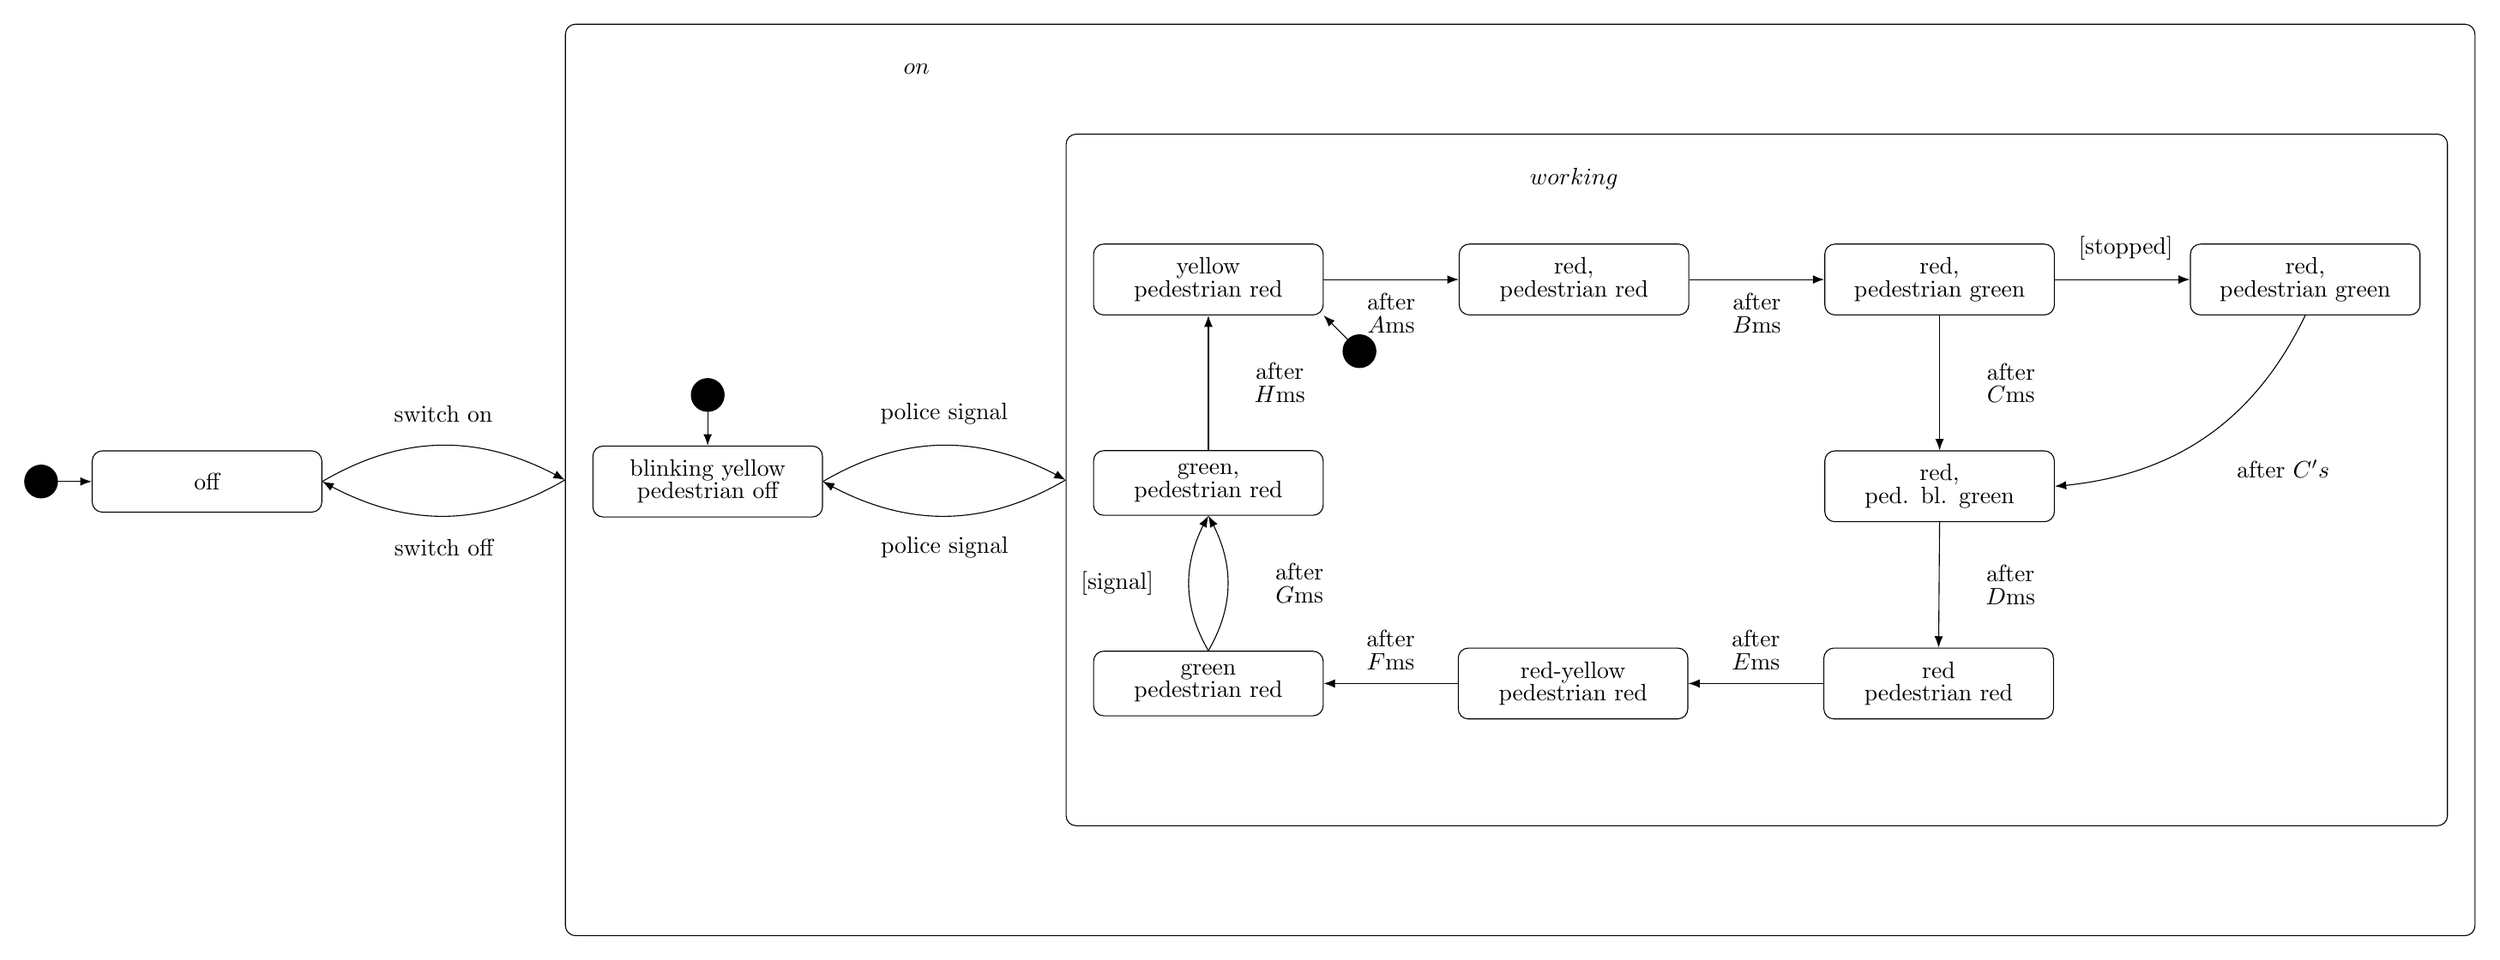
\begin{tikzpicture}[auto,
node distance = 22mm and 17mm,
every node/.style = {draw, rounded corners=1.5mm,
                     inner ysep=2mm, inner xsep=4mm,
                     minimum height=6ex,
                     text width=26mm, align=center},
                    ]
%---
\linespread{0.8}


\node (off) {off};

\node (by) [right=40mm of off] {blinking yellow \\ pedestrian off};
\node (by_a) [draw=none,above=20mm of by] {};
\node (by_d) [draw=none,below=20mm of by] {};

\node (y) [right=40mm of by_a] {yellow \\ pedestrian red};
\node (r_pr) [right=20mm of y] {red, \\ pedestrian red};
\node (r_pg) [right=20mm of r_pr] {red, \\ pedestrian green};
\node (r_pg_bl) [below=20mm of r_pg] {red, \\ ped. bl. green};
\node (g) [right=40mm of by_d] {green \\ pedestrian red};
\node (r_pr_2) [right=74mm of g] {red \\ pedestrian red};
\node (ry) [left=20mm of r_pr_2] {red-yellow \\ pedestrian red};

\node (r_pg_stopped) [right=20mm of r_pg] {red, \\ pedestrian green};
\node (g_signal) [above=20mm of g] {green, \\ pedestrian red};

\node (empty) [draw=none,right=0mm of r_pg,text width=3mm] {};
\node (working_label) [draw=none,above=5mm of r_pr] {$working$};
\node (working_label_2) [draw=none,below=5mm of g] {};
\node (working) [fit=(y)(r_pr)(r_pg)(r_pr_2)(ry)(g)(empty)(working_label)(working_label_2)(r_pg_stopped)(g_signal)] {};
\node (on_label) [draw=none,above left=5mm and 5mm of working] {$on$};
\node (on_label_2) [draw=none,below left=5mm and 5mm of working] {};
\node (on) [fit=(by)(working)(on_label)(on_label_2)] {};

\coordinate[above=10mm of by]   (temp1);
\coordinate[below right=10mm of y.south east]     (temp2);
\coordinate[left=10mm of off.west]   (temp3);
\path[{Circle[length=5mm,flex]}-{Latex[flex]}]
        (temp1) edge (by)
        (temp2) edge (y.south east)
        (temp3) edge (off.west);
\path[-{Latex[]},bend left]
        (off.east) edge node[draw=none,above] {switch on}  (on.west)
        (on.west) edge node[draw=none,below] {switch off} (off.east)

        (by.east) edge node[draw=none,above] {police signal} (working.west)
        (working.west) edge node[draw=none,below] {police signal} (by.east);
        
\path[-{Latex[]},]
        (y.east) edge node[draw=none,below,text width=13mm] {after $A$ms} (r_pr.west)
        (r_pr.east) edge node[draw=none,below,text width=13mm] {after $B$ms} (r_pg.west)
        (r_pg.south) edge node[draw=none,text width=13mm] {after $C$ms} (r_pg_bl.north)
        (r_pg.east) edge node[draw=none,text width=13mm] {[stopped]} (r_pg_stopped.west)
        (r_pg_stopped.south) edge [bend left] node[draw=none,text width=15mm] {after $C's$} (r_pg_bl.east)
        (r_pg_bl.south) edge node[draw=none,text width=13mm] {after $D$ms} (r_pr_2.north)
        (r_pr_2.west) edge node[draw=none,above,text width=13mm] {after $E$ms} (ry.east)
        (ry.west) edge node[draw=none,above,text width=13mm] {after $F$ms} (g.east)
        (g.north) edge [bend right]  node[draw=none,right,text width=13mm] {after $G$ms} (g_signal.south)
        (g.north) edge [bend left]   node[draw=none,left,text width=13mm] {[signal]} (g_signal.south)
        (g_signal.north) edge node[draw=none,right,text width=13mm] {after $H$ms} (y.south);


\end{tikzpicture}
    \end{document}
